%% manuscript.tex
%% Budget-Constrained Evaluation of Open-Weight LLM Agents:
%% Success-Budget Curves and Cost-Aware Model Selection
%%
%% Target venues (Elsevier): Information Processing & Management / ESWA / EAAI
%% Document class: elsarticle (see elsarticle.cls in this directory)
%%
%% Structure and section placeholders only -- body text to be filled in
%% after translation from the Chinese draft. Each section/subsection
%% contains a %TODO marker indicating what content belongs there.

\documentclass[preprint,12pt]{elsarticle}

%% ---------------------------------------------------------------
%% Packages
%% ---------------------------------------------------------------
\usepackage{amssymb}
\usepackage{amsmath}
\usepackage{graphicx}
\usepackage{booktabs}
\usepackage{multirow}
\usepackage{url}

%% Path to the figures produced by experiments/analysis/output/figures/
%% (relative to this .tex file at 稿件/latex/manuscript.tex)
\graphicspath{{../../experiments/analysis/output/figures/}}

\journal{Expert Systems with Applications}

\begin{document}

\begin{frontmatter}

%% ---------------------------------------------------------------
%% Title
%% ---------------------------------------------------------------
\title{Budget-Constrained Evaluation of Open-Weight LLM Agents: Success--Budget Curves, Price Reversal, and Thinking-Budget Saturation}

%% ---------------------------------------------------------------
%% Authors and affiliations (placeholders)
%% ---------------------------------------------------------------
\author[label1]{Author One}
\affiliation[label1]{organization={Affiliation Placeholder, Department Placeholder},
            addressline={Address Placeholder},
            city={City Placeholder},
            postcode={Postcode Placeholder},
            state={State/Province Placeholder},
            country={Country Placeholder}}

%% Add \ead{email@example.com} and \cortext / corref for corresponding
%% author once real author information is available.

%% ---------------------------------------------------------------
%% Abstract
%% ---------------------------------------------------------------
\begin{abstract}
Public leaderboards rank large language model (LLM) agents by success rate under an unlimited inference budget, whereas budget-sensitive practitioners face a different question: \emph{which model should be deployed when each task may spend at most a budget $B$?} We propose a budget-constrained evaluation protocol that treats the per-task budget as the independent variable and reports the success--budget curve $S(B)$ together with a family of derived metrics: the normalized area under the curve (AUBC), the budget-to-target $B_{@\tau}$, budget elasticity, and pairwise crossover points between models. We further show that for budget-unaware agents, the entire curve can be derived offline from a single maximum-budget run per task, decoupling evaluation cost from the number of budget levels. Applying the protocol to a coverage gap in existing evaluations---open-weight models served through public APIs---we evaluate 12 configurations of the DeepSeek-V4 and Qwen3 families (spanning a roughly 100-fold price range) on the three $\tau^3$-bench customer-service domains, collecting 4,448 multi-turn tool-use trajectories. Four findings emerge. (1) Budget constraints substantially reorder the leaderboard: at 0.3$\times$ the median budget-to-50\%-success, budget-constrained rankings are statistically unrelated to unconstrained ones (Kendall $\tau$ from $-0.02$ to $0.52$), and the budget required to reach 50\% success differs by 17--20$\times$ between models of comparable unconstrained accuracy. (2) The price-reversal phenomenon reported for single-turn reasoning does not appear in any of 66 model pairs (95\% upper confidence bound 4.4\%), because trajectory cost is dominated by repeatedly resent context rather than thinking tokens. (3) Thinking yields a real but strongly saturating benefit: a same-backbone paired contrast is significant ($p=0.0027$) at roughly twice the cost, yet the gain saturates at a budget of about 1K thinking tokens. (4) Open-weight hosted endpoints exhibit deterministic empty-response failures on up to 28\% of tasks for one model; treating these as infrastructure errors rather than model failures would inflate its measured success by 24 percentage points. All trajectories, code, and per-token cost records are released.
\end{abstract}

\begin{keyword}
LLM agents \sep evaluation benchmarks \sep inference cost \sep budget-constrained evaluation \sep open-weight models \sep tool use
\end{keyword}

\end{frontmatter}

%% =================================================================
\section{Introduction}
\label{sec:introduction}
Large language model (LLM) agents are moving from demonstrations to deployments. In customer service, software engineering, and scientific computing, an agent completes a task through many rounds of tool calls, and its inference consumption accumulates with every step: a single agentic task can cost tens of times more than a single-turn query. For budget-sensitive deployers---precisely the primary audience of open-weight models---the operative question is not \emph{which model is strongest} but \emph{which model should be deployed under a per-task budget $B$}.

Current evaluation practice cannot answer this question. Mainstream agent leaderboards report task success as the sole headline metric, and even the most recent cost-transparent infrastructure, the Holistic Agent Leaderboard (HAL)~\cite{kapoor2025holisticagentleaderboard}, records cost \emph{post hoc} rather than imposing it as a \emph{prospective constraint}: it reports what each model spent without limit, not what each model could still accomplish under a cap. The distinction is not rhetorical. Per-task costs of multi-step agents are heavy-tailed---in our data, costs for the same model within one domain span an order of magnitude---so mean cost conceals how budget truncation systematically affects the expensive tail. Meanwhile, single-turn reasoning studies have documented a \emph{price reversal} phenomenon, where models with lower list prices end up costlier due to highly variable thinking-token usage~\cite{chen2026pricereversal}; that work explicitly calls for treating inference cost as a first-class evaluation dimension and extending the analysis to agentic settings, but whether the phenomenon amplifies or vanishes over multi-step trajectories has remained an open empirical question.

This paper proposes a \emph{budget-constrained evaluation protocol} for LLM agents. The protocol treats a hard per-task budget cap $B$ as the independent variable of evaluation and reports the success--budget curve $S(B)$ along with a family of derived metrics: the normalized area under the budget curve (AUBC) as a scalar cost-effectiveness summary; the budget-to-target $B_{@\tau}$, i.e., the minimum budget at which success reaches $\tau$; the budget elasticity $\varepsilon(B)$; and the set of pairwise \emph{crossover points} between the curves of any two models, which directly yields a budget-interval-to-best-model lookup table and turns model selection into a table lookup. The protocol rests on a simple but consequential observation: for an agent that is unaware of its budget, the trajectory under any budget $B$ is exactly the prefix of its maximum-budget trajectory truncated where cumulative cost first exceeds $B$. Consequently, \emph{a single maximum-budget run per task suffices} to derive $S(B)$ at every budget level offline, decoupling evaluation cost from the number of budget levels.

We apply the protocol to a coverage gap in current evaluations: \emph{open-weight models served through public APIs}. Using the three customer-service domains of $\tau^3$-bench~\cite{barres2025tau2bench} (airline, retail, telecom; 278 tasks in total) as the testbed, we evaluate 12 model configurations from the DeepSeek-V4 and Qwen3 families, spanning a roughly 100-fold price range, dense and mixture-of-experts architectures, and thinking and non-thinking modes, with the user simulator and judge fixed across all runs for comparability. This coverage is complementary to HAL (nine closed frontier models, no Chinese open-weight models), and for budget-sensitive deployers these models constitute the realistic candidate set.

The results support the necessity of the protocol. At 0.3$\times$ the median budget-to-50\%-success, budget-constrained rankings are statistically unrelated to the unconstrained success ranking in two domains (airline: Kendall $\tau=-0.02$, $p=0.94$; retail: $\tau=0.17$, $p=0.46$), recovering agreement only at 3$\times$ the median budget ($\tau=0.60$--$0.88$, $p<0.01$). To reach 50\% success, the most cost-effective model (Qwen3.5-27B) needs \$0.010--\$0.015 per task while the flagship Qwen3.7-Max needs \$0.18--\$0.26---a 17--20$\times$ gap at essentially equal unconstrained accuracy. The price reversal reported for 21.8\% of model pairs in single-turn settings appears in none of our 66 pairs: trajectory cost is dominated by repeatedly resent context (input-to-output token ratios of roughly 10:1 to 40:1), which dilutes the thinking-token variance that drives the single-turn effect. A thinking-budget sweep yields a clearly saturating dose--response: the benefit of thinking is confirmed by a same-backbone paired contrast ($p=0.0027$) but saturates at about 1K thinking tokens, with a 16-fold larger budget buying only two further percentage points.

Our contributions are as follows.
\begin{enumerate}
\item \textbf{Protocol and metrics.} To our knowledge, the first prospective budget-constrained evaluation protocol for multi-step agents, comprising the $S(B)$/AUBC/$B_{@\tau}$/elasticity/crossover metric family, the single-run curve derivation, and a task-level paired-bootstrap inference procedure.
\item \textbf{Coverage and artifacts.} To our knowledge, the first systematic cost--capability study of Chinese open-weight agent models (12 configurations $\times$ 3 domains $\times$ 278 tasks; 4,448 valid multi-turn trajectories), with all trajectories and per-token cost records released.
\item \textbf{Findings.} Quantitative evidence that budgets reorder agent leaderboards; a mechanistic account of why single-turn price reversal disappears in multi-step tasks; a saturating dose--response curve for thinking budgets; and a systematic empty-response failure mode of open-weight hosted endpoints, with its consequences for evaluation accounting.
\end{enumerate}

%% =================================================================
\section{Related Work}
\label{sec:related-work}
\paragraph{Agent benchmarks.} $\tau$-bench and its successor $\tau^3$-bench~\cite{barres2025tau2bench} characterize customer-service agents through LLM-simulated users and policy-constrained tool calls; the $\tau^3$ release fixed more than 75 task defects identified by SABER~\cite{cuadron2025saber} and added a telecom domain, making it one of the most strictly scored multi-turn tool-use benchmarks available. SWE-bench~\cite{jimenez2024swebench}, GAIA~\cite{mialon2023gaia}, and AgentBench~\cite{liu2024agentbench} cover software engineering and general assistance, typically with ReAct-style agents~\cite{yao2023react}. Across all of these, leaderboards rank by success rate; cost appears at most as a footnote.

\paragraph{Cost-aware evaluation.} Kapoor et al.~\cite{kapoor2025aiagentsmatter} first argued that agent evaluations neglect cost, proposed joint accuracy--cost Pareto reporting, and showed that simple baselines often Pareto-dominate elaborate agents; their follow-up HAL~\cite{kapoor2025holisticagentleaderboard} standardized evaluation infrastructure and recorded the cost of nine closed frontier models across nine benchmarks (21{,}730 rollouts, \$40K). Cost-of-Pass~\cite{erol2025costofpass} defines the expected monetary cost per correct solution and tracks its frontier over model releases. The closest motivation to ours is the price-reversal study~\cite{chen2026pricereversal}: on nine single-turn reasoning datasets, 21.8\% of model pairs invert between list-price order and realized-cost order, driven by thinking-token variance (up to 9.7$\times$ for a repeated query), and the authors call for cost as a first-class evaluation dimension. \emph{Our difference from all of the above lies in the evaluation semantics}: they record or aggregate realized spending, whereas we impose a prospective budget constraint and measure the response of success to budget---the former answers ``how much was spent,'' the latter answers ``what can be accomplished under a given budget,'' which is the form deployment decisions take. BCAS~\cite{mccleary2026budgetconstrainedsearch} ablates design decisions of retrieval agents under fixed budgets but is restricted to one scaffold family and does not propose curve-family metrics; Efficient Agents~\cite{wang2025efficientagents} reduces agent cost by design rather than measuring cross-model budget response.

\paragraph{Test-time compute and thinking budgets.} Overthinking and adaptive test-time compute have been surveyed systematically~\cite{alomrani2025reasoningonabudget}, and adaptive effort selection has been studied for agents~\cite{yang2026ares}. Public APIs now expose thinking-budget controls, turning the amount of thinking into a controllable experimental variable; existing measurements, however, focus on single-turn mathematics and coding, and the dose--response of thinking budget on multi-step agent success had not been measured systematically (our RQ3).

\paragraph{Open-weight and production evaluation.} Mainstream agent leaderboards contain almost no Chinese open-weight models, although their roughly order-of-magnitude lower unit prices make them the de facto option for budget-sensitive deployments; production-oriented surveys likewise identify cost efficiency as a missing dimension of current evaluation frameworks~\cite{mehta2025enterpriseagenticframework}. This paper provides the first systematic cost--capability data for these models on a strictly scored multi-turn benchmark.

%% =================================================================
\section{Budget-Constrained Evaluation Protocol}
\label{sec:protocol}

\subsection{Problem Formulation}
\label{subsec:problem-formulation}
Let agent $m$ produce trajectory $\tau(m,x)$ on task $x$, where the $i$-th model call consumes $p_i$ input tokens and $c_i$ output tokens (thinking tokens included, matching API billing). Given list prices $(\alpha_{\mathrm{in}}, \alpha_{\mathrm{out}})$ in USD per million tokens (cache-miss rates), the incremental cost of step $i$ is $\kappa_i = (\alpha_{\mathrm{in}}\, p_i + \alpha_{\mathrm{out}}\, c_i)/10^{6}$ and the cumulative cost is $K_j = \sum_{i \le j} \kappa_i$. The outcome of task $x$ under budget $B$ is
\begin{equation}
\mathrm{succ}_B(m,x) = 1 \iff \text{the trajectory terminates naturally, is scored successful, and } K(m,x) \le B.
\end{equation}
\emph{Accounting boundary.} The budget constrains only the evaluated agent's own calls; the user simulator and the judge are evaluation infrastructure whose costs are reported separately and excluded from $B$. All experiments fix the user simulator (DeepSeek-V4-Flash) and judge (DeepSeek-V4-Pro) to keep models strictly comparable.

\subsection{Deriving Full Curves from Single Runs}
\label{subsec:deriving-curves}
\begin{proposition}[Truncation equivalence]
If an agent is budget-unaware---its policy does not condition on the remaining budget---then its trajectory under budget $B$ equals the prefix of its maximum-budget trajectory truncated where cumulative cost first exceeds $B$.
\end{proposition}
The claim follows directly from budget-independence of the policy: the per-step decision distribution is identical under both conditions, and the only difference is the external truncation time. As a corollary, $S(B)$ for every $B$ can be computed offline from one maximum-budget run per task, making evaluation cost independent of the number of budget levels. Budget-\emph{aware} agents violate the premise and require one run per budget level; we leave them to future work (Section~\ref{sec:discussion}).

\subsection{Metric Family}
\label{subsec:metric-family}
On a per-domain logarithmically spaced budget grid (200 points spanning $[0.5\times$ the minimum completed-trajectory cost, $1.05\times$ the maximum$]$) we define:
\begin{itemize}
\item $S(B) = \mathbb{E}_x[\mathrm{succ}_B(m,x)]$: the success--budget curve, nondecreasing in $B$ with $S(\infty) = \mathrm{pass@1}$;
\item $\mathrm{AUBC} = \int S \, d\log B \,/\, \Delta \log B \in [0,1]$: a scalar summary of low-budget usability and high-budget ceiling;
\item $B_{@\tau} = \min \{B : S(B) \ge \tau\}$: the budget-to-target, directly usable in deployment service-level objectives;
\item elasticity $\varepsilon(B) = d\log S / d\log B$: the marginal return of budget;
\item crossover points $B^{*}(m_1, m_2)$: budgets at which $S_1$ and $S_2$ intersect with a sign change, yielding a budget-interval-to-best-model lookup table.
\end{itemize}
\emph{Statistical inference.} Within a domain all models face the same task set, so all between-model comparisons use task-level \emph{paired} bootstrap (2{,}000 resamples, fixed seed) for 95\% confidence intervals; rank stability across budget levels is quantified with Kendall's $\tau$ (nine tests; all significance conclusions survive Holm correction). One anchor model per provider tier is run with three independent trials to estimate run-to-run variance as a reference for interpreting single-run differences.

\subsection{Research Questions}
\label{subsec:research-questions}
\begin{itemize}
\item \textbf{RQ1.} How do $S(B)$ curves differ across models, and does the unconstrained leaderboard remain informative at low budgets? Where are the crossover points?
\item \textbf{RQ2.} Does the single-turn price-reversal phenomenon persist at trajectory level---do cheaper list prices still predict cheaper realized costs after thinking-token variance accumulates over many steps?
\item \textbf{RQ3.} What is the dose--response of thinking budget (0/1K/4K/16K tokens) on multi-step task success and cost?
\end{itemize}
In addition to these pre-registered questions, data collection surfaced an unanticipated reliability phenomenon of open-weight hosted endpoints, which we report in Section~\ref{subsec:reliability-failures} together with its accounting implications. Budget-aware agents, which violate the truncation-equivalence premise of Section~\ref{subsec:deriving-curves}, are left to future work.

%% =================================================================
\section{Experimental Setup}
\label{sec:experimental-setup}

\subsection{Testbed}
\label{subsec:testbed}
We use the three text domains of $\tau^3$-bench~\cite{barres2025tau2bench}: airline (50 tasks), retail (114), and telecom (114), with the default \texttt{base} split and official scoring (database-state matching plus natural-language assertions). The domains represent the most common deployed agent form---multi-turn tool use under policy constraints---with largely deterministic scoring, and the $\tau^3$ release incorporates over 75 task fixes~\cite{cuadron2025saber}. To probe generalization beyond this task family, we conduct a validation experiment on BFCL multi-turn function calling as a second benchmark family (Section~\ref{sec:results}).

\subsection{Model Matrix}
\label{subsec:model-matrix}
We evaluate 12 configurations, all served through public Chinese APIs (Table~\ref{tab:table1-main} lists them): DeepSeek-V4 (flash/pro), Qwen3.7 (max/plus), Qwen3.6-flash, the open-weight Qwen3.5 series (397B-A17B, 122B-A10B, 35B-A3B, 27B), Qwen3-32B, and the same-backbone contrast pair Qwen3-235B-A22B (instruct vs.\ thinking). List prices span roughly two orders of magnitude (input prices from CNY 0.4 to 12 per million tokens). Qwen3-32B is run with \texttt{enable\_thinking=false} due to a DashScope non-streaming restriction and billed at its non-thinking rate. The complete price table with source URLs and verification dates is released with the code (\texttt{models.yaml}). For RQ3, Qwen3.6-flash is swept over thinking budgets of 0 (disabled), 1{,}024, 4{,}096, and 16{,}384 tokens on the airline domain, with three trials for the 0 and 1{,}024 arms.

\subsection{Cost Accounting and Reproducibility}
\label{subsec:cost-accounting}
Cost equals token counts times official list prices (cache-miss rates, verified 2026-07-04); CNY prices are converted at the CFETS mid rate of 6.8067 (2026-07-01). \emph{List-price versus realized billing.} Under this accounting, the agent-side cost of all experiments is \$177.5, whereas the actual bills of the two providers total approximately CNY 825 ($\approx$\$121); the gap stems from provider-side context-cache discounts (a 93.5\% input-cache hit rate on DeepSeek, with hit prices roughly 1/120 of miss prices), limited-time promotions, and free quotas. Because such discounts vary with deployment patterns and are not reproducible, list-price accounting is our primary metric, with realized billing data released alongside. All runs use temperature 0; the user simulator and judge are fixed throughout; two judge components of the $\tau^3$-bench harness that default to an OpenAI model were patched to DeepSeek-V4-Pro (patch released). Deterministic empty-response failures of an evaluated model are counted as task failures of that model (Section~\ref{subsec:reliability-failures}); the two empty responses of the user simulator (evaluation infrastructure) are excluded from denominators and reported. Per-step token and cost sequences for every trajectory, all code, and analysis scripts are released.

%% =================================================================
\section{Results}
\label{sec:results}

\subsection{Budget Reshuffles the Leaderboard}
\label{subsec:budget-reshuffles}
%TODO: Present Table~\ref{tab:table1-main} and Figure~\ref{fig:sb-curves};
% discuss rank instability of the pass@1 leaderboard as the budget
% threshold B varies; reference Kendall's tau rank-correlation analysis
% (fig3\_kendall.txt / fig3\_rank\_table.csv) if retained in the final
% narrative.

\begin{figure}[t]
\centering
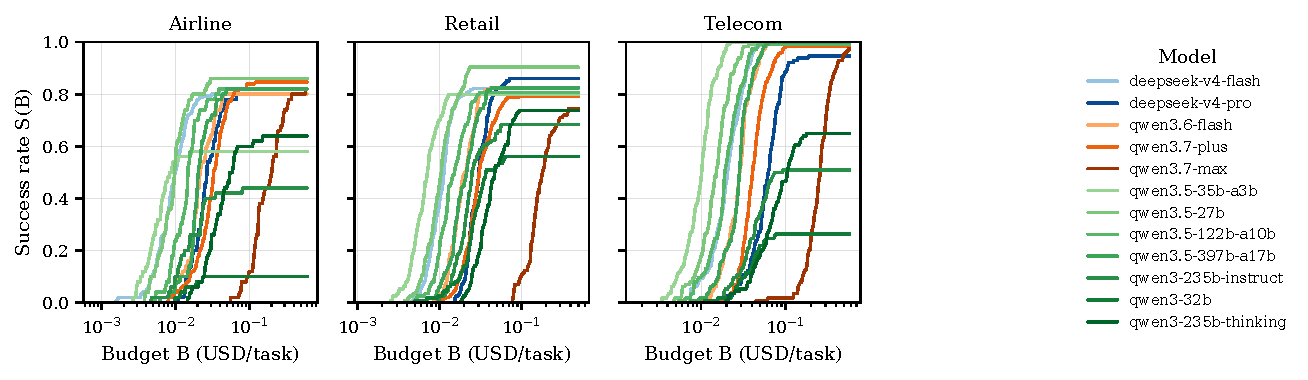
\includegraphics[width=\linewidth]{fig1_sb_curves.pdf}
%TODO: finalize caption text.
\caption{Success-budget (S-B) curves across the model matrix.}
\label{fig:sb-curves}
\end{figure}

\subsection{Absence of Price Reversal in Multi-Step Tasks}
\label{subsec:price-reversal}
%TODO: Present Figure~\ref{fig:aubc-vs-price}; discuss whether the price
% reversal phenomenon (cheaper reasoning models costing more at
% comparable capability, cf. Chen et al. 2026) is or is not observed in
% multi-step agentic tasks, and why.

\begin{figure}[t]
\centering
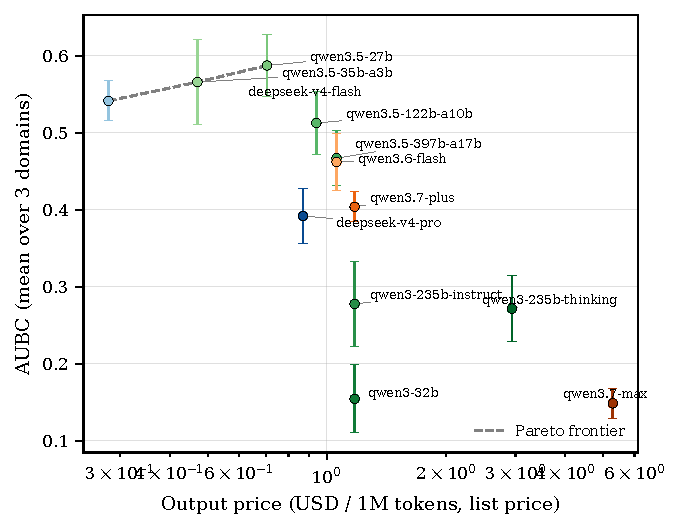
\includegraphics[width=\linewidth]{fig2_aubc_vs_price.pdf}
%TODO: finalize caption text.
\caption{AUBC versus list price across models.}
\label{fig:aubc-vs-price}
\end{figure}

\subsection{Thinking-Budget Dose--Response}
\label{subsec:dose-response}
%TODO: Discuss the dose-response relationship between thinking-token
% budget and (a) success rate, (b) realized cost, across the
% thinking-mode model variants (e.g., qwen3-235b-thinking vs.
% qwen3-235b-instruct).

\subsection{Reliability Failures of Open-Weight Endpoints}
\label{subsec:reliability-failures}
%TODO: Present Figure~\ref{fig:price-vs-realized}; discuss the gap
% between list/quoted price and realized per-episode cost, endpoint
% failures, timeouts, and other reliability issues encountered with
% open-weight model API providers during data collection.

\begin{figure}[t]
\centering
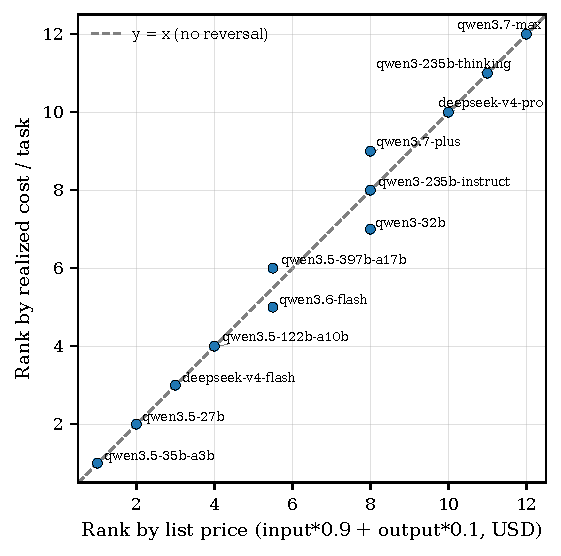
\includegraphics[width=\linewidth]{fig4_price_vs_realized.pdf}
%TODO: finalize caption text.
\caption{Quoted price versus realized cost per episode.}
\label{fig:price-vs-realized}
\end{figure}

%% -----------------------------------------------------------------
%% Table 1 skeleton, derived from
%% experiments/analysis/output/table1_main.csv
%% Columns: model, domain, n_valid, pass1, mean_cost_usd,
%%          aubc_with_ci95, b_at_50_usd, b_at_80_usd
%% -----------------------------------------------------------------
\begin{table}[t]
\centering
%TODO: finalize caption; define all columns and abbreviations (pass@1,
% AUBC with 95\% CI, budget-at-50/80\% success in USD).
\caption{Main results across the model matrix and tau2-bench domains.}
\label{tab:table1-main}
\begin{tabular}{l l r r r c r r}
\toprule
Model & Domain & $n_{\text{valid}}$ & pass@1 & Mean cost (USD) & AUBC [95\% CI] & $B_{@50}$ (USD) & $B_{@80}$ (USD) \\
\midrule
%TODO: populate data rows from table1_main.csv, e.g.:
%TODO: deepseek-v4-flash & airline & 150 & 0.8000 & 0.010109 & 0.5156 [0.4732, 0.5575] & 0.009984 & 0.031032 \\
%TODO: deepseek-v4-flash & retail  & 342 & 0.8216 & 0.010543 & 0.5354 [0.5089, 0.5619] & 0.011521 & 0.021049 \\
%TODO: deepseek-v4-flash & telecom & 342 & 0.9942 & 0.022311 & 0.5738 [0.5644, 0.5834] & 0.020661 & 0.031118 \\
%TODO: ... (remaining models: deepseek-v4-pro, qwen3-235b-instruct,
%TODO:      qwen3-235b-thinking, qwen3-32b, qwen3.5-122b-a10b,
%TODO:      qwen3.5-27b, qwen3.5-35b-a3b, qwen3.5-397b-a17b,
%TODO:      qwen3.6-flash, qwen3.7-max, qwen3.7-plus; include AVERAGE rows)
%TODO: consider \multirow for model names spanning domain rows, or a
%TODO: separate summary table restricted to AVERAGE rows for the main text.
\bottomrule
\end{tabular}
\end{table}

%% =================================================================
\section{Discussion and Limitations}
\label{sec:discussion}
%TODO: Synthesize findings across 5.1-5.4; discuss threats to validity
% (single-run curve reconstruction, provider pricing volatility,
% generalization beyond tau2-bench domains, sample sizes per domain);
% discuss implications for practitioners doing cost-aware model
% selection; discuss limitations relative to Holistic Agent Leaderboard
% / AI Agents That Matter recommendations for rigorous agent evaluation.

%% =================================================================
\section{Conclusion}
\label{sec:conclusion}
%TODO: Summarize contributions (budget-constrained evaluation protocol,
% single-run curve derivation method, empirical findings on open-weight
% agents) and future work (broader domains, additional providers,
% dynamic/adaptive budget allocation).

%% =================================================================
%% Bibliography
%% =================================================================
\bibliographystyle{elsarticle-num}
\bibliography{refs}

\end{document}
